\documentclass[tikz,border=8pt]{standalone}
\usepackage{amsmath}
\usetikzlibrary{positioning,arrows.meta}
\definecolor{navy}{HTML}{0D3555}
\definecolor{blue}{HTML}{1670AD}
\definecolor{teal}{HTML}{278168}
\definecolor{gold}{HTML}{E8A420}
\definecolor{light}{HTML}{F4F7FA}
\begin{document}
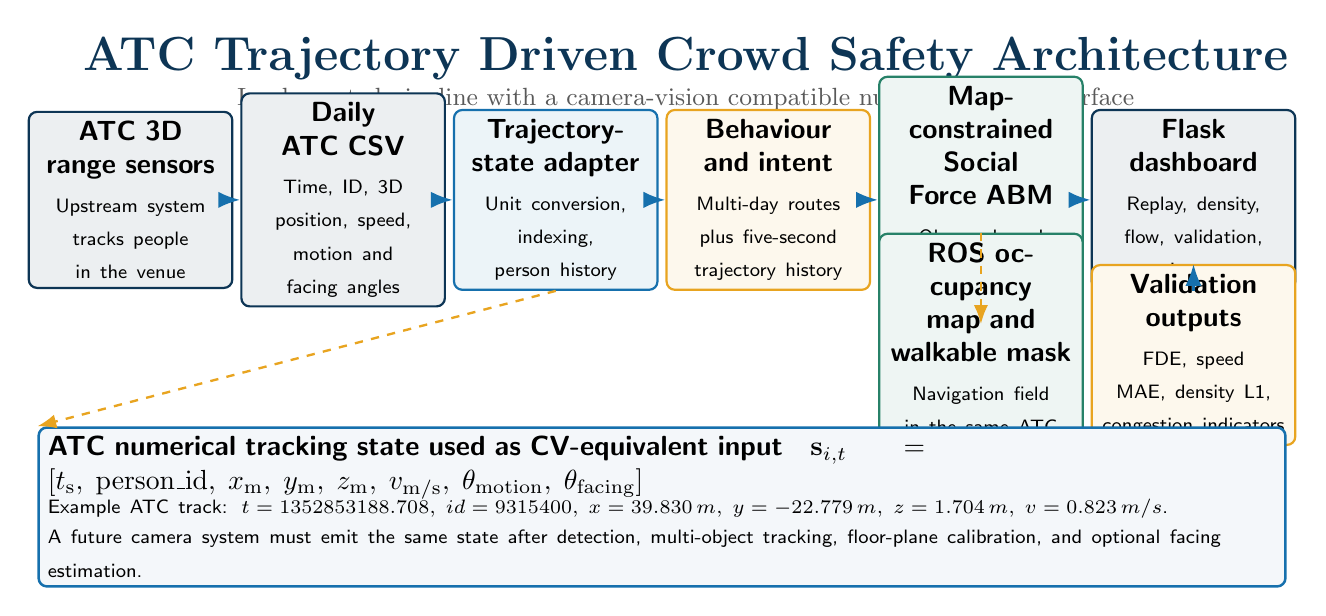
\begin{tikzpicture}[
  font=\sffamily,
  box/.style={draw=#1, fill=#1!8, rounded corners=3pt, line width=0.8pt, minimum height=1.25cm, text width=2.35cm, align=center},
  flow/.style={-Latex, line width=1.1pt, draw=blue},
  support/.style={-Latex, line width=0.85pt, draw=gold, dashed}
]

\node[font=\bfseries\LARGE, text=navy] at (8.4,6.55) {ATC Trajectory Driven Crowd Safety Architecture};
\node[font=\small, text=black!65] at (8.4,6.03) {Implemented pipeline with a camera-vision compatible numerical state interface};

\node[box=navy] (sensor) at (1.35,4.75) {\textbf{ATC 3D range sensors}\\[2pt]\scriptsize Upstream system tracks people in the venue};
\node[box=navy] (csv) at (4.05,4.75) {\textbf{Daily ATC CSV}\\[2pt]\scriptsize Time, ID, 3D position, speed, motion and facing angles};
\node[box=blue] (adapter) at (6.75,4.75) {\textbf{Trajectory-state adapter}\\[2pt]\scriptsize Unit conversion, indexing, person history};
\node[box=gold] (profile) at (9.45,4.75) {\textbf{Behaviour and intent}\\[2pt]\scriptsize Multi-day routes plus five-second trajectory history};
\node[box=teal] (abm) at (12.15,4.75) {\textbf{Map-constrained Social Force ABM}\\[2pt]\scriptsize Observed seed or synthetic capacity scenario};
\node[box=navy] (ui) at (14.85,4.75) {\textbf{Flask dashboard}\\[2pt]\scriptsize Replay, density, flow, validation, capacity outputs};

\draw[flow] (sensor) -- (csv);
\draw[flow] (csv) -- (adapter);
\draw[flow] (adapter) -- (profile);
\draw[flow] (profile) -- (abm);
\draw[flow] (abm) -- (ui);

\node[box=teal] (map) at (12.15,2.78) {\textbf{ROS occupancy map and walkable mask}\\[2pt]\scriptsize Navigation field in the same ATC coordinate frame};
\node[box=gold] (validation) at (14.85,2.78) {\textbf{Validation outputs}\\[2pt]\scriptsize FDE, speed MAE, density L1, congestion indicators};
\draw[support] (map) -- (abm);
\draw[flow] (ui) -- (validation);

\node[draw=blue, fill=light, rounded corners=3pt, line width=0.9pt, minimum height=1.35cm, text width=15.6cm, align=left] (state) at (8.1,0.85) {
\textbf{ATC numerical tracking state used as CV-equivalent input}\quad
\(\mathbf{s}_{i,t}=[t_{\mathrm{s}},\;\mathrm{person\_id},\;x_{\mathrm{m}},\;y_{\mathrm{m}},\;z_{\mathrm{m}},\;v_{\mathrm{m/s}},\;\theta_{\mathrm{motion}},\;\theta_{\mathrm{facing}}]\)\\[-1pt]
\scriptsize Example ATC track: \(t=1352853188.708,\;id=9315400,\;x=39.830\,m,\;y=-22.779\,m,\;z=1.704\,m,\;v=0.823\,m/s\).\\[-1pt]
\scriptsize A future camera system must emit the same state after detection, multi-object tracking, floor-plane calibration, and optional facing estimation.};
\draw[support] (adapter.south) -- (state.north west);
\end{tikzpicture}
\end{document}
